\documentclass{home_assignment}
\usepackage{booktabs,caption}
\usepackage{tikz}
 \usetikzlibrary{shapes, arrows,  positioning}
   \tikzstyle{active} = [rectangle, text width=2cm, minimum height=2cm,    text centered, draw=black, fill=green!20]
   \tikzstyle{failed} = [rectangle, text width=2cm, minimum height=2cm,    text centered, draw=black, fill=red!20]
   \tikzstyle{arrow} = [thick,->,>=stealth]
   \newcommand{\countinfinity}[1]{
    \def\argI{1}%
    \def\argII{0}%
    \def\temp{#1}%
   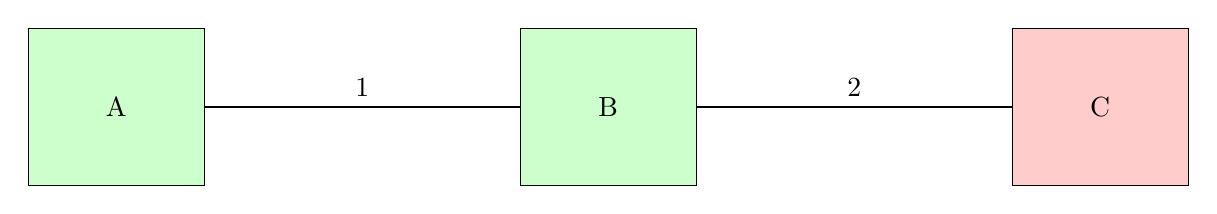
\begin{tikzpicture}[node distance=4cm]
   \node (a) [active] {A};
   \node (b) [active, right=of a] {B};
   \draw [arrow,-] (a) -- node[anchor=south]{1} (b);
   \ifx\temp\argI
   \node (c) [active, right=of b] {C};
   \draw [arrow,-] (b) -- node[anchor=south]{2} (c);
   \fi

   \ifx\temp\argII
   \node (c) [failed, right=of b] {C};
   \fi
  \end{tikzpicture}
   }

   \newcommand{\counttable}[5]{
    \def\argI{1}%
    \def\argII{0}%
    \def\temp{#1}%
    \begin{tikzpicture}[node distance=2cm]
     \node(a){%
     \begin{tabular}{ccc}
        \multicolumn{3}{c}{A}\\
        \hline
        To & Cost & Via\\
        \hline 
        B & 1 & B\\
        C & \textcolor{red}{#2} & \textcolor{red}{#3}\\
        \hline 
        \end{tabular}
     };
     \node (b)[right=of a]{%
     \begin{tabular}{ccc}
        \multicolumn{3}{c}{B}\\
        \hline
        To & Cost & Via\\
        \hline 
        A & 1 & A\\
        C & \textcolor{red}{#4} & \textcolor{red}{#5}\\
        \hline 
        \end{tabular}
     };

     \ifx\temp\argI
     \node (c)[right=of b]{%
     \begin{tabular}{ccc}
        \multicolumn{3}{c}{C}\\
        \hline
        To & Cost & Via\\
        \hline 
        A & 3 & B\\
        B & 2 & B\\
        \hline 
        \end{tabular}
     };
     \fi

     \ifx\temp\argII
     \node (c)[right=of b]{%
     \begin{tabular}{ccc}
        \multicolumn{3}{c}{C}\\
        \hline
        To & Cost & Via\\
        \hline 
        A & - & -\\
        B & - & -\\
        \hline 
        \end{tabular}
     };
     \fi
    \end{tikzpicture}
   }

\begin{document}
\titlePage{Computer Networks Assignment \#3}{December 12, 2020}{Sharad Kumar Ghimire}
\newcounter{departmentCounter}
\setcounter{departmentCounter}{0}
\newcommand{\calculateaddress}[1]{
\addtocounter{departmentCounter}{1}
\begin{table}[H]
 \centering
 \begin{tabular}{C{3cm}C{2.5cm}C{2.5cm}C{2.5cm}C{2.5cm}}
\toprule
#1
\bottomrule
 \end{tabular}
 \caption{Calculation for network address and broadcast of subnet \Alph{departmentCounter}}
\end{table}
}
\problem{List out typical features of the following networking devices:}
\subproblem{Repeater}
Repeater is a networking device that regenerates signal over the network so that the length of transmission can be extended without the signal becoming too weak or corrupted. 
\begin{itemize}
\item A repeater operates at the physical layer.
\item It is a 2 port device.
\item Doesn't amplify the signal, rather copies the signal bit by bit and regenerates it at the original strength.
\end{itemize}

\subproblem{Hub}
Hub is a networking device that is used to connect different branches of wires or devices.
\begin{itemize}
\item A hub operates at the physical layer.
\item Hub can't filter data packets, meaning that the packets are sent to all the connected devices except the sender.
\item It acts as a multiport repeater and hence regenerates and retransmits the received signal to all the connected destination without intelligent path sorting. 
\end{itemize}

\subproblem{Bridge}
Bridge is a networking device that is used to connect two LANs working with the same protocol. 
\begin{itemize}
\item A bridge operates at the data link layer.
\item It is a 2 port device.
\item Bridge is a repeater with additional feature of filtering content with the help of physical address of the source and destination using the flooding and forwarding principle. In this, the bridge records the response from devices to the data it broadcasts after sending it to any host. Based on this, the data is properly sent to the destination host it was meant for.
\end{itemize}

\subproblem{Switch}
Switch acts as a multiport bridge with a buffer.
\begin{itemize}
\item A switch operates at the data link layer.
\item It can perform error checking prior to data forwarding.
\end{itemize}

\subproblem{Router}
A router is a networking device used to route data packets to destination hosts based on the IP addresses from the routing table. 
\begin{itemize}
\item A router operates at the network layer.
\item It has multiple interfaces, all of which have a unique IP address to connect to different subnets of a larger network.
\item It divides the broadcast domains of the hosts that are connected through it.
\end{itemize}

\subproblem{Gateway}
Gateway is the gate or a passage that connects two networks that maybe working with different protocols.
\begin{itemize}
\item A gateway operates at all the 5 layers.
\item It is the last destination from where data packets leave the autonomous system, or the first destination from where the packets enter the autonomous system.
\item It can perform protocol conversion.
\end{itemize}
\problem{Why is a logical address necessary for network communication, though there is unique
physical address? Explain.}
Logical address is a CPU generated virtual address that is essential in network routing. On the other hand, a physical address is used by the memory management unit to access a particular memory cell. In networking terms, a logical address is the IP address whereas a physical address is the MAC address of a device on the network. The MAC address is company defined and can't be changed by the user. Devices whose only last octet of the MAC address vary can be located in completely different geographical locations based on when and where they were bought, sold or distributed. If we were to use the physical address of a device to communicate over a network, the signal must be broadcasted all over the globe to properly detect the true destination by listening to the response of the devices. On the other hand, a unique logical address can be used to effectively pinpoint the desired destination on the network hence establishing an easy communication route since an IP address is logical and routable address.\\ IP address is a combination of network and host address parts along with a structured subnet mask. The logical routing can be performed based on the network address which means the router needs to store minimal information about the destinations to forward the packets, hence making logical addressing necessary for network communication despite having a unique physical address.

\problem{What is private and public IP address? How can a network having private addresses be connected with the global Internet? Explain.}
Private IP address of a host device is the IP address that is used by other devices within the same local network as the host to address the host. It is only visible to the devices within the same local network and thus can't be accessed publicly. IP address in the blocks 100.0.0.0/24, 172.16.0.0/20 and 192.168.0.0/16 are private ip addresses. Likewise, the public IP address of a host device is the IP address that is used by devices outside the local network of the host to address the host. It is visible outside the local network meaning that servers on the vast internet can locate a public IP address. \\
A network with private addresses can be connected to the global Internet with the use of NAT capabilities of the router the network has as the gateway device. Internet Service Providers (ISPs) allocate certain public IP addresses to the routers they distribute as a part of the service connection. In general, a private network is connected to these routers that have a public IP as provided by the ISPs which are then connected to some upstream routers that eventually lead to a connection with the internet. Once data packets are sent from a host within the private network, the router receives these packets and performs SNAT on them which replaces the private IP address of the host with its own public IP address. These data packets that are now addressed as the public IP of the router make their wahy on to the global Internet. Whenever the flow has to be reversed, the packets are sent to the public IP of the router which is visible from the Internet. The router then performs NAT on the data packets hereby replacing the public IP address of the router with the private address of the actual sending host device. 

\problem{What is subnetting? Why is it important in networking? Explain with suitable examples.}
Subnetting is a logical process by which a larger TCP/IP network is divided or subnetted into smaller networks called subnets for easy management purposes. It is achieved using a four octet or 32-bit number called a subnet mask.\\
The importance of subnetting can be understood with a real-life analogy. Consider an organization, for instance say a campus that has access to a private network given by the address 192.168.1.0/24 which means that there are 254 available IP addresses in the major network. If there are three departments that need IP addresses to assign to host devices within the department and we wish to provide separate subnets to each of the departments, we can achieve this with a subnet mask 255.255.255.192, i.e. /26 in slash notation. This divides the main network 192.168.1.0/24 into three subnets namely A, B and C. Each of these subnets has 62 possible host IP addresses, one network address each as 192.168.1.0, 192.168.1.64 and 192.168.1.128 and one broadcast address each as 192.168.1.63, 192.168.1.127 and 192.168.1.191 respectively. This essentially divides the main network into separate subnets with separate management capabilities. This also reduces network congestion with network traffic being isolated in the subnet that it originated in, but still providing a cross subnet communication.

\problem{Suppose you have given the IP address of 102.5.4.0/23 for your company. There are five different departments having 200, 100, 40, 20 and 12 hosts. Two additional point-to-point links are there for interconnection between routers. Divide the given IP address for above requirements. List out the network address, broadcast address, usable IP address range and subnet mask of each subnet.}
Since there are 5 deparments that need different number of host devices, we'll be subnetting the main network 102.5.4.0/23 into five subnets namely A, B, C, D and E for the deparments and one additional subnet for the two point-to-point interconnection between routers. The main network supports 510 IP addresses, out of which we need 374 addresses. 
\subsubsection*{Subnet A}
Department A needs 200 hosts but since it isn't achievable directly, we'll need to allocate 254 usable host addresses, plus two IP addresss, one for network address and one for broadcast address in the subnet A.
For this, the subnet mask to be used is /24, and the network address can be calculated as,
\calculateaddress{Decimal notation & 102 & 5 & 4 & 0\\
\midrule
Binary notation & 0110 0110 & 0000 0101 & 0000 0100 & XXXX XXXX\\}
For the network address, the Xs are replaced by 0 giving us 102.5.4.0. Likewise, for the broadcast address the Xs are replaced by 1 giving us 102.5.4.255. The usable range of IP addresses is 102.5.4.1 to 102.5.4.254, giving us 254 possible hosts where one is used for the router interface from the subnet and the required 200 hosts can be connected to the subnet with 53 hosts to spare.
\\
Since we've used 256 address for department A, the other IP addresses belong to the network 102.5.5.0/24. 
\subsubsection*{Subnet B}
Department B needs 100 hosts but since it isn't achievable directly, we'll need to allocate 126 usable host addresses, plus two IP addresss, one for network address and one for broadcast address in the subnet B.
For this, the subnet mask to be used is /25, and the network address can be calculated as,
\calculateaddress{Decimal notation & 102 & 5 & 5 & 0\\
\midrule
Binary notation & 0110 0110 & 0000 0101 & 0000 0101 & 0XXX XXXX\\}
For the network address, the Xs are replaced by 0 giving us 102.5.5.0. Likewise, for the broadcast address the Xs are replaced by 1 giving us 102.5.5.127. The usable range of IP addresses is 102.5.5.1 to 102.5.5.126, giving us 126 possible hosts where one is used for the router interface from the subnet and the required 100 hosts can be connected to the subnet with 25 hosts to spare.
\subsubsection*{Subnet C}
Department C needs 40 hosts but since it isn't achievable directly, we'll need to allocate 62 usable host addresses, plus two IP addresss, one for network address and one for broadcast address in the subnet C.
For this, the subnet mask to be used is /26, and the network address can be calculated as,
\calculateaddress{Decimal notation & 102 & 5 & 5 & 128\\
\midrule
Binary notation & 0110 0110 & 0000 0101 & 0000 0101 & 10XX XXXX\\}
For the network address, the Xs are replaced by 0 giving us 102.5.5.128. Likewise, for the broadcast address the Xs are replaced by 1 giving us 102.5.5.191. The usable range of IP addresses is 102.5.5.129 to 102.5.5.190, giving us 62 possible hosts where one is used for the router interface from the subnet and the required 40 hosts can be connected to the subnet with 21 hosts to spare.
\subsubsection*{Subnet D}
Department D needs 20 hosts but since it isn't achievable directly, we'll need to allocate 30 usable host addresses, plus two IP addresss, one for network address and one for broadcast address in the subnet D.
For this, the subnet mask to be used is /27, and the network address can be calculated as,
\calculateaddress{Decimal notation & 102 & 5 & 5 & 192\\
\midrule
Binary notation & 0110 0110 & 0000 0101 & 0000 0101 & 110X XXXX\\}
For the network address, the Xs are replaced by 0 giving us 102.5.5.192. Likewise, for the broadcast address the Xs are replaced by 1 giving us 102.5.5.223. The usable range of IP addresses is 102.5.5.193 to 102.5.5.222, giving us 30 possible hosts where one is used for the router interface from the subnet and the required 20 hosts can be connected to the subnet with 9 hosts to spare.
\subsubsection*{Subnet E}
Department E needs 12 hosts but since it isn't achievable directly, we'll need to allocate 14 usable host addresses, plus two IP addresss, one for network address and one for broadcast address in the subnet E.
For this, the subnet mask to be used is /28, and the network address can be calculated as,
\calculateaddress{Decimal notation & 102 & 5 & 5 & 224\\
\midrule
Binary notation & 0110 0110 & 0000 0101 & 0000 0101 & 1110 XXXX\\}
For the network address, the Xs are replaced by 0 giving us 102.5.5.224. Likewise, for the broadcast address the Xs are replaced by 1 giving us 102.5.5.239. The usable range of IP addresses is 102.5.5.225 to 102.5.5.238, giving us 14 possible hosts where one is used for the router interface from the subnet and the required 10 hosts can be connected to the subnet with 3 hosts to spare.
\subsubsection*{Subnet F}
The two additional point-to-point connections for routers also require a subnet of two hosts, and since it is achievable exactly, we allocate 2 usage host addresses, plus two IP addresss, one for network address and one for broadcast address in the subnet F.
For this, the subnet mask to be used is /30, and the network address is 102.5.5.240. Likewise, for the broadcast address is 102.5.5.243.
\subsubsection*{Overall subnet division}
\begin{table}[H]
\centering
\begin{tabular}{|C{1cm}||C{2cm}||C{2.5cm}||C{2.5cm}||C{3cm}||C{1cm}|}
 \hline
 Subnet&Required Hosts&Network Address&Broadcast Address&
 Usable IP Addresses&Subnet Mask\\
 \hline
 A & 200 & 102.5.4.0 & 102.5.4.255 & 102.5.4.1-102.5.4.254 & /24\\
 \hline
 B & 100 & 102.5.5.0 & 102.5.5.127 & 102.5.5.1-102.5.5.126 & /25\\
 \hline
 C & 40 & 102.5.5.128 & 102.5.5.191 & 102.5.5.129-102.5.5.190 & /26\\
 \hline
 D & 20 & 102.5.5.192 & 102.5.5.223 & 102.5.5.193-102.5.5.222 & /27\\
 \hline
 E & 12 & 102.5.5.224 & 102.5.5.239 & 102.5.5.225-102.5.5.238 & /28\\
 \hline
 F & 2 & 102.5.5.240 & 102.5.5.243 & 102.5.5.241-102.5.5.242& /30\\
 \hline
\end{tabular}
\caption{Subnet division as required by Problem 5}
\end{table}
\problem{What is the count to infinity problem in distance vector routing? How can it be addressed? Explain with example.}
\begin{figure}[H]
    \centering
    \countinfinity{1}
    \caption{Router connections with certain node costs when no link is down}
    \label{fig:counta}
  \end{figure}

  \begin{figure}[H]
    \centering
   \counttable{1}{3}{B}{2}{C}
    \caption{Routing tables for A, B and C when no link is down}
    \label{fig:counttbla}
  \end{figure}
Consider three routers A, B and C as shown in Figure~\ref{fig:counta} where the numbers on the link represent the cost metric for getting from one router to the other. Figure~\ref{fig:counttbla} shows the routing tables for A, B and C where the entries for To, Cost and Via are set according to the Figure~\ref{fig:counta}.
\begin{figure}[H]
    \centering
    \countinfinity{0}
    \caption{Router connections with certain node costs when link between B and C is down}
    \label{fig:countb}
  \end{figure}

  \begin{figure}[H]
    \centering
   \counttable{0}{3}{B}{2}{C}
    \caption{Routing tables for A, B and C when link between B and C is down}
    \label{fig:counttblb}
  \end{figure}
Now if we consider that the router C goes down and loses its link with B, as shown in Figure~\ref{fig:countb}. Also, Figure~\ref{fig:counttblb} shows the routing tables when the link is down.
\begin{figure}[H]
    \centering
   \counttable{0}{3}{B}{4}{A}
    \caption{Routing tables for A, B and C when link between B and C is down and B updates with the routing information from A}
    \label{fig:counttblc}
  \end{figure}
  When B realizes the direct link to C is down, it updates the routing table using the routing table for A. Figure~\ref{fig:counttblc} shows the updated routing tables where the router B looks for a link to C via A with the cost of 4.
  \begin{figure}[H]
    \centering
   \counttable{0}{5}{B}{4}{A}
    \caption{Routing tables for A, B and C when link between B and C is down and A updates with the routing information from B}
    \label{fig:counttbld}
  \end{figure}
  Once B has updated the routing table, it sends the updated information to its neighbors where A realizes that the entry for C has changed, and hence updates its own routing table for the entry to reach C via B with the cost of 5 as shown in Figure~\ref{fig:counttbld}
  \begin{figure}[H]
    \centering
   \counttable{0}{5}{B}{6}{A}
    \caption{Routing tables for A, B and C when link between B and C is down and B updates with the routing information from A}
    \label{fig:counttble}
  \end{figure}
  Again, since A has updated the routing table, it sends the updated information to its neighbors where B realizes that the entry for C has changed, and hence updates its own routing table for the entry to reach C via A with the cost of 6 as shown in Figure~\ref{fig:counttble}.\\[\baselineskip]
  It is visible that the two routers A and B continuously try to find a link to the router C via each other and go on increasing their cost to infinity. The value of infinity is generally set to a high cost rather than the actual infinity sense. This problem where the routers update the cost to reach a router in the network goes to a very large value is called the cost to infinity problem.
  \subsubsection*{Split Horizon Technique}
  Split horizon technique is a method to address the cost to infinity problem. In this technique, a router won't inform about a route to a neighbor from which it initially received the route. In our case, the router B won't inform the updated route to the router A and hence the false information of having a link to the router C won't get transmitted. A will learn that there is no possible link to C in the next update and hence the problem won't occur.
  \subsubsection*{Route Poisoning Technique}
  Route poisoning technique is another way to mitigate the cost to infinity problem. In this technique, whenever a router finds out that a route is invalid/down, it tranmits the route with a metric that exceeds the maximum value. Say the maximum value of the cost metric is N in the above case, so when B detects the faulty route, it stores the route as a cost of N+1, which will notify router A that the link from B to C is invalid and hence A also removes the entry from its table.  
\problem{What is unicast, multicast and broadcast? How does multicast differ from multiple unicast? Why do routers not forward broadcast packets? Explain.}
\subsubsection*{Unicast}
Unicast is the transmission where only one sender and one receiver are involved, meaning that the data packets from the sender are sent to a single destination host. It is a one-to-one transmission and is one of the most common form of data transfer over the network.
\subsubsection*{Multicast}
Multicast is the transmission where one sender and multiple receivers are involved, meaning that the data packets from the sender are sent to multiple destination hosts. It is a one-to-many transmission.
\subsubsection*{Broadcast}
Broadcast is the transmission where one sender and all the receivers on the network are involved, meaning that the data packets from the sender are sent to all other devices on the network.
\\[\baselineskip]
The group of destination hosts that are to receive a data packet during a multicast transmission is valled multicast group. This group is identified by using a multicast address, which is the IP used by a sending host to send the data packets to the multicast group. The router handles the task of duplicating the data packets when necessary and transmit it to all the destinations on the multicast group. For this, the number of data packets actually on the network is less since all the multicast group is sent the packet using a single multicast address, whereas the router does most of the heavy task of sending the packets to individual host addressses. On the contrary, for multicast unicast transmission, the sender identifies the IP addresses of all the destination hosts and has to send the data packets to them individually itself. This causes the network to be over-populated by similar data packets with varying destinations thereby wasting network resources. The sending host has to perform majority of the task in this form of multicast transmission.
\\[\baselineskip]
A broadcast address is used for the broadcast transmission from a sender host to all the devices under the broadcast address. If routers were to forward broadcast packets then some senders could populate other networks with unnecessary data and make the network slow to respond due to increased traffic activity. A host in a different subnet could send unnecessary data to the broadcast address of another subnet without affecting the internal network but drastically affecting the other network, which is why the routers don't forward broadcast packets.

\problem{Differentiate:}
\subproblem{Distance vector routing vs. Link state routing}
\difference{Distance vector routing}{Link state routing}{
Bandwidth& Less due to smaller packets, no flooding and local sharing implementations. 
& More due to flooding and large packets that include link state information. \\ \hline
Updates based on& Neighbors information. 
& Global information. \\ \hline
Traffic& Less
& More\\ \hline
Count to infinity problem & Yes 
& No\\ \hline
Loops& Persistent loops 
& Transient loops\\ \hline
Algorithm used& Bellman Ford
& Dijkstra\\ \hline
Practical implementation& RIP and IGRP
& OSPF and ISIS\\ \hline
}
\subproblem{IGP vs. EGP}
\difference{IGP}{EGP}{
 Abbreviation & Interior Routing Protocol & Exterior Routing Protocol\\ \hline
 Working & Send routing table and information between routers that are in the same internet network. & Send routing information between different networks. \\ \hline
 Implemented& Within the network as well as in gateways.& Only on the gateways. \\ \hline
 Available protocols & RIP, OSPF, ISIS, EIGRP & BGP\\ \hline
}
\subproblem{SNAT vs. DNAT}
\difference{SNAT}{DNAT}{
    Abbreviation               & Source Network Address Translation & Destination Network Address Translation \\ \hline
    Initiating source location & Inside the network.                & Outside the network.                    \\ \hline
    IP modification            & Source IP address is modified.     & Destination IP address is modified.     \\ \hline
}
\subproblem{ARP vs. RARP}
\difference{ARP}{RARP}{
    Abbreviation     & Address Resolution Protocol                                     & Reverse Address Resolution Protocol                                    \\ \hline
    Usage            & Used to find MAC address of a host device using the IP address. & Used to request the IP address of a host device using the MAC address. \\ \hline
    Relevance        & Still in use.                                                   & Obsolete and replaced by DHCP.                                         \\ \hline
    Table managed at & Local host.                                                     & RARP server.                                                           \\ \hline
}

\problem{Discuss briefly on:}
\subproblem{RIP}
RIP, abbreviation for Routing Information Protocol, is an Internal Gateway Protocol (IGP) that makes use of the distance vector algorithm to maintain the routing tables. Number of hops is selected as the metric for the algorithm with the maximum being set to 15, which is used to diminish the count to infinity problem by utilizing route poisoning and split horizon techniques. 
\\
There are mainly two versions of the RIP that have been used, viz. RIPv1 and RIPv2. The first version of RIP made use of broadcast messages to transfer the routing information. Additionally, this form of RIP didn't exchange subnet information and thus it doesn't support VLSM. The second version of RIP made use of multicast messaging to transfer the routing information and also shares the subnet information allowing VLSM to be implemented.
\subproblem{OSPF}
OSPF, abbreviation for Open Shortest Path First, is a link state routing algorithm that uses flooding to transfer link state information. It makes use of Dijkstra's shortest path algorithm to locate the shorest path for each subnet on the network. A router making use of OSPF stores the information of the entire network where the link costs are set by the administrator. It then applies the shortest path algorithm with itself as the starting node. The routing information is shared using broadcast messaging whenever there is a change in the link state or at a fixed interval even if no changes are detected. 
\subproblem{BGP}
BGP, abbreviation for Border Gateway Protocol is the only available Exterior Gateway Protocol (EGP). It makes use of path vector routing which is a variant of the distance vector routing. Routers executing on the BGP store cost of a path to destination networks and intermediate autonomous systems where the metrics for the path vector are calculated based on policies set rather than using the hop count as in RIP. To avoid the count to infinity and looping problems the router sends routing information to another router with its own AS number included so that whenever it can check for routing loops by verfying if its AS number is present or not. 
\subproblem{ICMP}
ICMP, abbreviation for Internet Control Message Protocol is used for reporting errors and management queries between networking devices. It is used to report errors in the network layers, such as TTL of an IP datagram expiring, destination host being unrechable and so on. Since IP doesn't have a pre-built-in mechanism for exchanging such information, ICMP is used as a supporting protocol to exchange these informations. ICMP messages include a type and a code to denote the information it represents. Ping program makes use of the ICMP messages where a host receiving an ICMP echo request replies with a echo reply to test connectivity status between the hosts.
\end{document}